%% Advances in Space Research submission (Elsevier elsarticle).
%% All numbers in the text are macros defined in numbers.tex, which is
%% generated from the pipeline outputs by src/asr/make_numbers.py.
\documentclass[final,5p,times,twocolumn,authoryear]{elsarticle}

\usepackage{amsmath,amssymb}
\usepackage{graphicx}
\usepackage{booktabs}
\usepackage{siunitx}
\usepackage{hyperref}
\usepackage[switch,columnwise]{lineno}
\usepackage[capitalize]{cleveref}
\hypersetup{colorlinks=true,linkcolor=blue,citecolor=blue,urlcolor=blue}
\linenumbers
\modulolinenumbers[5]
\renewcommand{\topfraction}{0.9}
\renewcommand{\dbltopfraction}{0.9}
\renewcommand{\textfraction}{0.07}
\renewcommand{\floatpagefraction}{0.75}
\renewcommand{\dblfloatpagefraction}{0.75}
\setcounter{dbltopnumber}{3}

% DOIs as https://doi.org/... links (ASR guide reference examples)
\newcommand{\DOIprefix}{}
\AtBeginDocument{\providecommand{\doi}[1]{}\renewcommand{\doi}[1]{\href{https://doi.org/#1}{\path{https://doi.org/#1}}}}
% AUTO-GENERATED by src/asr/make_numbers.py -- do not edit
\newcommand{\AlSunlit}{31.8}
\newcommand{\AlUmbra}{0.16}
\newcommand{\CeilAl}{0.87}
\newcommand{\CeilAlvTwo}{0.57}
\newcommand{\CeilMg}{0.75}
\newcommand{\CovAllArea}{100.0}
\newcommand{\CovFiveArea}{99.7}
\newcommand{\CovUsedArea}{100.0}
\newcommand{\CovUsedCells}{100.00}
\newcommand{\FootprintA}{37}
\newcommand{\FootprintB}{25}
\newcommand{\FwhmAlDec}{185}
\newcommand{\GainDec}{13.74}
\newcommand{\GainPctDec}{1.8}
\newcommand{\GoesTmedFive}{5.1}
\newcommand{\GoesTmedFour}{5.5}
\newcommand{\GoesTmedSix}{5.3}
\newcommand{\GrsAlCI}{[0.66, 0.76]}
\newcommand{\GrsAlCIvOne}{[0.13, 0.28]}
\newcommand{\GrsAlCIvTwo}{[0.26, 0.44]}
\newcommand{\GrsAlN}{1{,}790}
\newcommand{\GrsAlR}{0.72}
\newcommand{\GrsAlRMinK}{0.72}
\newcommand{\GrsAlRMinKKK}{0.69}
\newcommand{\GrsAlRho}{0.60}
\newcommand{\GrsAlRvOne}{0.21}
\newcommand{\GrsAlRvTwo}{0.35}
\newcommand{\GrsMgCI}{[0.56, 0.66]}
\newcommand{\GrsMgCIvTwo}{[0.54, 0.65]}
\newcommand{\GrsMgN}{1{,}790}
\newcommand{\GrsMgR}{0.61}
\newcommand{\GrsMgRMinK}{0.58}
\newcommand{\GrsMgRMinKKK}{0.58}
\newcommand{\GrsMgRho}{0.63}
\newcommand{\GrsMgRvTwo}{0.60}
\newcommand{\GrsSitesAl}{-0.34}
\newcommand{\GrsSitesMg}{-0.11}
\newcommand{\GzAlCI}{[0.66, 0.77]}
\newcommand{\GzAlMed}{0.91}
\newcommand{\GzAlR}{0.72}
\newcommand{\GzAlRel}{0.96}
\newcommand{\GzMgCI}{[0.49, 0.61]}
\newcommand{\GzMgMed}{0.23}
\newcommand{\GzMgR}{0.56}
\newcommand{\GzMgRel}{0.76}
\newcommand{\GzN}{295{,}814}
\newcommand{\GzPct}{51}
\newcommand{\GzSiteAlCI}{[0.55, 0.97]}
\newcommand{\GzSiteAlR}{0.80}
\newcommand{\GzSiteAlRFive}{0.43}
\newcommand{\GzSiteAlROne}{0.75}
\newcommand{\GzSiteMgCI}{[$-$0.78, 0.88]}
\newcommand{\GzSiteMgR}{0.15}
\newcommand{\GzSiteMgRFive}{-0.19}
\newcommand{\GzSiteMgROne}{-0.62}
\newcommand{\LineFracMgHi}{80}
\newcommand{\LineFracMgLo}{63}
\newcommand{\LineFracSiHi}{74}
\newcommand{\LineFracSiLo}{55}
\newcommand{\MapThi}{8.0}
\newcommand{\MapTlo}{3.6}
\newcommand{\MapTmed}{5.2}
\newcommand{\MedAl}{0.92}
\newcommand{\MedAlvTwo}{0.82}
\newcommand{\MedGrsAl}{0.71}
\newcommand{\MedGrsMg}{0.58}
\newcommand{\MedMg}{0.22}
\newcommand{\MedRelAl}{0.96}
\newcommand{\NConverged}{1{,}037{,}846}
\newcommand{\NDayside}{1{,}053{,}989}
\newcommand{\NGoesOK}{1{,}017{,}226}
\newcommand{\NHeaderSample}{4{,}800}
\newcommand{\NMapped}{578{,}530}
\newcommand{\NMappedMinK}{143{,}961}
\newcommand{\NMappedMinKKK}{11{,}259}
\newcommand{\NMappedvTwo}{429{,}217}
\newcommand{\NMonths}{24}
\newcommand{\NRawFiles}{1{,}515{,}239}
\newcommand{\NStackDec}{75{,}707}
\newcommand{\NSunlitDec}{8{,}555}
\newcommand{\NUmbraDec}{2{,}254}
\newcommand{\OffsetDec}{2.2}
\newcommand{\OldGrsAl}{0.19}
\newcommand{\OldGrsMg}{0.48}
\newcommand{\PassMaxMonth}{June 2025}
\newcommand{\PassMaxPct}{71}
\newcommand{\PassMedPct}{50}
\newcommand{\PassMinMonth}{January 2021}
\newcommand{\PassMinPct}{0}
\newcommand{\PctAllSCD}{74}
\newcommand{\PctFullExp}{99.4}
\newcommand{\PctMapped}{54.9}
\newcommand{\PctNotAllSCD}{26}
\newcommand{\PctPartialExp}{0.6}
\newcommand{\PfiveAl}{0.49}
\newcommand{\PfiveMg}{0.07}
\newcommand{\PninetyfiveAl}{1.38}
\newcommand{\PninetyfiveMg}{0.43}
\newcommand{\RelAl}{0.97}
\newcommand{\RelAlvTwo}{0.42}
\newcommand{\RelGrsAl}{0.78}
\newcommand{\RelGrsMg}{0.73}
\newcommand{\RelMg}{0.76}
\newcommand{\RelMgvTwo}{0.82}
\newcommand{\RhoAlGoes}{0.39}
\newcommand{\RhoAlHard}{0.06}
\newcommand{\RhoAlSoft}{0.75}
\newcommand{\SecMaxPct}{1.3}
\newcommand{\SigmaZeroDec}{74}
\newcommand{\SiteAlFiveBias}{+0.218}
\newcommand{\SiteAlFiveCI}{[$-$0.36, 0.89]}
\newcommand{\SiteAlFiveLooHi}{0.63}
\newcommand{\SiteAlFiveLooLo}{0.30}
\newcommand{\SiteAlFiveR}{0.47}
\newcommand{\SiteAlFiveRho}{0.47}
\newcommand{\SiteAlFiveRhoP}{0.21}
\newcommand{\SiteAlFiveRmse}{0.240}
\newcommand{\SiteAlOneBias}{+0.240}
\newcommand{\SiteAlOneCI}{[0.51, 0.99]}
\newcommand{\SiteAlOneLooHi}{0.92}
\newcommand{\SiteAlOneLooLo}{0.66}
\newcommand{\SiteAlOneR}{0.71}
\newcommand{\SiteAlOneRho}{0.87}
\newcommand{\SiteAlOneRhoP}{0.00}
\newcommand{\SiteAlOneRmse}{0.253}
\newcommand{\SiteAlTwoBias}{+0.242}
\newcommand{\SiteAlTwoCI}{[0.48, 0.97]}
\newcommand{\SiteAlTwoCIvTwo}{[$-$0.08, 0.96]}
\newcommand{\SiteAlTwoLooHi}{0.86}
\newcommand{\SiteAlTwoLooLo}{0.81}
\newcommand{\SiteAlTwoR}{0.81}
\newcommand{\SiteAlTwoRho}{0.78}
\newcommand{\SiteAlTwoRhoP}{0.01}
\newcommand{\SiteAlTwoRmse}{0.252}
\newcommand{\SiteAlTwoRvTwo}{0.43}
\newcommand{\SiteFpMax}{200}
\newcommand{\SiteFpMin}{124}
\newcommand{\SiteMgFiveBias}{+0.033}
\newcommand{\SiteMgFiveCI}{[$-$0.80, 0.89]}
\newcommand{\SiteMgFiveLooHi}{0.56}
\newcommand{\SiteMgFiveLooLo}{-0.38}
\newcommand{\SiteMgFiveR}{0.09}
\newcommand{\SiteMgFiveRho}{0.20}
\newcommand{\SiteMgFiveRhoP}{0.61}
\newcommand{\SiteMgFiveRmse}{0.055}
\newcommand{\SiteMgOneBias}{+0.040}
\newcommand{\SiteMgOneCI}{[$-$0.96, $-$0.22]}
\newcommand{\SiteMgOneLooHi}{-0.51}
\newcommand{\SiteMgOneLooLo}{-0.85}
\newcommand{\SiteMgOneR}{-0.64}
\newcommand{\SiteMgOneRho}{-0.73}
\newcommand{\SiteMgOneRhoP}{0.02}
\newcommand{\SiteMgOneRmse}{0.068}
\newcommand{\SiteMgTwoBias}{+0.043}
\newcommand{\SiteMgTwoCI}{[$-$0.50, 0.83]}
\newcommand{\SiteMgTwoCIvTwo}{[$-$0.22, 0.88]}
\newcommand{\SiteMgTwoLooHi}{0.49}
\newcommand{\SiteMgTwoLooLo}{0.11}
\newcommand{\SiteMgTwoR}{0.38}
\newcommand{\SiteMgTwoRho}{0.17}
\newcommand{\SiteMgTwoRhoP}{0.67}
\newcommand{\SiteMgTwoRmse}{0.058}
\newcommand{\SiteMgTwoRvTwo}{0.37}
\newcommand{\SynColdAl}{+5 to +7}
\newcommand{\SynColdMg}{+28 to +33}
\newcommand{\SynHotAl}{+3 to +5}
\newcommand{\SynHotMg}{$-$15 to $-$13}
\newcommand{\SynMaxBiasMgAl}{4}
\newcommand{\SynPullHi}{1.25}
\newcommand{\SynPullLo}{0.84}
\newcommand{\TsensAlHi}{+8}
\newcommand{\TsensAlLo}{$-$9}
\newcommand{\TsensMgHi}{+27}
\newcommand{\TsensMgLo}{$-$25}
\newcommand{\XsmChiOne}{3.9}
\newcommand{\XsmChiTwo}{2.8}
\newcommand{\XsmNClass}{6{,}327}
\newcommand{\XsmNMin}{1{,}386}
\newcommand{\XsmNMonths}{3}
\newcommand{\XsmOneAl}{+4}
\newcommand{\XsmOneAlHi}{+8}
\newcommand{\XsmOneAlLo}{$-$1}
\newcommand{\XsmOneAlMA}{+3}
\newcommand{\XsmOneAlMB}{+5}
\newcommand{\XsmOneAlMC}{+2}
\newcommand{\XsmOneMg}{+14}
\newcommand{\XsmOneMgHi}{+32}
\newcommand{\XsmOneMgLo}{$-$1}
\newcommand{\XsmOneMgMA}{+14}
\newcommand{\XsmOneMgMB}{+15}
\newcommand{\XsmOneMgMC}{+12}
\newcommand{\XsmOneN}{6{,}256}
\newcommand{\XsmTRatio}{1.12}
\newcommand{\XsmTRatioHi}{1.17}
\newcommand{\XsmTRatioLo}{1.01}
\newcommand{\XsmTgoesMed}{5.6}
\newcommand{\XsmTmed}{6.2}
\newcommand{\XsmTwoAl}{$-$4}
\newcommand{\XsmTwoAlHi}{+1}
\newcommand{\XsmTwoAlLo}{$-$11}
\newcommand{\XsmTwoAlMA}{$-$6}
\newcommand{\XsmTwoAlMB}{$-$2}
\newcommand{\XsmTwoAlMC}{$-$6}
\newcommand{\XsmTwoMg}{$-$21}
\newcommand{\XsmTwoMgHi}{$-$3}
\newcommand{\XsmTwoMgLo}{$-$42}
\newcommand{\XsmTwoMgMA}{$-$24}
\newcommand{\XsmTwoMgMB}{$-$15}
\newcommand{\XsmTwoMgMC}{$-$27}
\newcommand{\XsmTwoN}{6{,}100}


\journal{Advances in Space Research}

\begin{document}

\begin{frontmatter}

\title{Global Mg/Si and Al/Si maps of the Moon from Chandrayaan-2 CLASS with time-resolved solar excitation from GOES XRS}

\author[ind]{Paidi Geetesh Chandra\corref{cor1}}
\ead{paidigeeteshchandra@gmail.com}
\author[ind]{Smarak Kanjilal}
\author[ind]{Subarno Maji}
\cortext[cor1]{Corresponding author. All authors contributed equally to this work.}
\affiliation[ind]{organization={Independent Researcher},addressline={IIT Kharagpur},postcode={721302},state={West Bengal},country={India}}

\begin{abstract}
We describe a processing chain for spectra of the Chandrayaan-2 Large Area Soft X-ray Spectrometer (CLASS) that uses only public data. Each \SI{8}{s} spectrum is fitted on raw counts with a Poisson likelihood and a simplified fundamental-parameter model: primary fluorescence with matrix effects and incidence geometry, scattered solar X-rays, detector and filter response, and a particle background. The incident solar spectrum is approximated by an isothermal CHIANTI spectrum at the temperature measured by the GOES X-Ray Sensor (XRS) for each exposure. Because solar lines carry \LineFracSiLo--\LineFracMgHi\% of the flux that excites Mg, Al and Si, element/Si ratios depend appreciably on this spectrum. We also describe an instrumental Al K$\alpha$ component that appears when the spacecraft is sunlit from behind and whose treatment in the background model affects Al/Si. In synthetic tests Mg/Si and Al/Si are recovered with small biases, whereas Ca/Si, Ti/Si and Fe/Si are not constrained with this approach. From \NRawFiles{} exposures in \NMonths{} monthly archives, \NMapped{} spectra pass pre-declared quality criteria and give global 2\textdegree{} maps with quality layers and no infill. Al/Si correlates with the Lunar Prospector Gamma-Ray Spectrometer (GRS) on 5\textdegree{} pixels ($r=\GrsAlR$) and with nine landing-site soils ($r=\SiteAlTwoR$). Mg/Si correlates with GRS ($r=\GrsMgR$), but its landing-site comparison is inconclusive. Refitting up to \XsmNClass{} overlapping spectra from three months with solar spectra from the Chandrayaan-2 Solar X-ray Monitor changes the median Al/Si by \XsmTwoAl{} to \XsmOneAl\% and Mg/Si by \XsmTwoMg{} to \XsmOneMg\%, within the stated systematic uncertainties.

\end{abstract}


\begin{keyword}
Moon \sep X-ray fluorescence \sep Chandrayaan-2 CLASS \sep solar X-ray spectrum \sep GOES XRS \sep lunar surface composition
\end{keyword}

\end{frontmatter}

\section{Introduction}\label{sec:intro}

The major-element chemistry of the lunar surface records how the crust formed and evolved. Highland plagioclase is rich in Al and Ca; mare basalts are rich in Fe, Mg and Ti. Global maps of these elements constrain magma-ocean crystallisation, mare volcanism and impact mixing \citep{Heiken1991}. Orbital gamma-ray spectroscopy has provided global maps of Fe, Ti, Th and K, and model-dependent estimates of Mg, Al, Si and Ca, at a resolution of hundreds of kilometres \citep{Lawrence1998,Prettyman2006}.

X-ray fluorescence (XRF) excited by solar X-rays offers better spatial resolution and direct sensitivity to Mg, Al and Si \citep{Jenkins1999,Beckhoff2006}. The Chandrayaan-1 X-ray Spectrometer (C1XS) demonstrated the technique during a period of very low solar activity, when only a few flares gave usable spectra \citep{Grande2009,Narendranath2011}. Its successor on Chandrayaan-2, the Large Area Soft X-ray Spectrometer (CLASS), has a geometric area of \SI{64}{cm^2} and a footprint of $\approx$\SI{12.5}{km} \citep{Narendranath2014,Narendranath2020,Pillai2021}. It has operated through the rise of solar cycle 25, and its Level-1 spectra are public.

Turning XRF line intensities into composition requires the spectrum of the incident solar X-rays. The fluorescence yield of each element depends on the solar flux above its absorption edge. A softer or harder solar spectrum therefore changes line ratios such as Mg/Si or Ca/Si even when the surface composition is unchanged. The Chandrayaan-2 Solar X-ray Monitor (XSM) measures this spectrum \citep{Mithun2020}, and the instrument team's analyses combine CLASS spectra with simultaneous XSM data. For users without an XSM-based workflow, the usual fallback is to assume a reference solar spectrum or to rely on line ratios. Ratios do not remove the dependence on the solar spectrum, because each element samples a different part of it.

In this paper we develop and validate a CLASS processing chain that can be reproduced entirely from public data, without XSM spectra. We take the solar excitation from the GOES X-Ray Sensor: its two-channel temperature, applied to isothermal CHIANTI spectra, gives a time-resolved solar spectrum for every CLASS exposure. Our specific contributions are:
\begin{enumerate}
\item a simplified fundamental-parameter forward model (Sherman primary fluorescence with matrix attenuation and incidence geometry, scattered solar spectrum, binned Gaussian detector response), fitted to raw counts by Poisson maximum likelihood with per-spectrum uncertainties, goodness of fit and quality flags;
\item the identification of a solar-driven instrumental Al K$\alpha$ component in CLASS spectra, present only when the spacecraft is sunlit, and a two-template background model that separates it from the particle background;
\item a quantified error budget from synthetic recovery tests, including the bias caused by errors in the solar temperature, which shows which element ratios can and cannot be recovered without a measured solar spectrum;
\item global Mg/Si and Al/Si maps from \NMonths{} monthly archives, with observation-count and uncertainty layers, validated against returned-sample compositions at nine landing sites and against Lunar Prospector GRS maps, using analysis choices fixed before validation.
\end{enumerate}
We report element ratios relative to Si, not absolute abundances, and we state explicitly which quantities the data cannot constrain.

\section{Data}\label{sec:data}

\subsection{CLASS Level-1 spectra}\label{sec:class}
The Chandrayaan-2 Large Area Soft X-ray Spectrometer (CLASS) carries sixteen e2v CCD-236 swept-charge devices (SCDs) of \SI{4}{cm^2} each, behind a collimator that defines a ground footprint of $\approx$\SI{12.5}{km} from the nominal \SI{100}{km} orbit \citep{Narendranath2014,Pillai2021}. We use the publicly released Level-1 product from the PRADAN portal of the Indian Space Science Data Centre. Each Level-1 file is an OGIP pulse-height table of 2048 channels holding the counts summed over the SCDs listed in the \texttt{SCD\_USED} keyword for one \SI{8}{s} integration, together with the four footprint corner coordinates, the solar incidence angle \texttt{SOLARANG}, the emission angle \texttt{EMISNANG}, the exposure time, detector temperature and the processing-software version.

We downloaded every monthly archive available to us: \NMonths{} archives (December 2020; January and February 2021; March 2022; March 2024; and every month from November 2024 to May 2026), totalling \NRawFiles{} Level-1 exposures. The archives are non-contiguous because CLASS observes only when the spacecraft attitude, power and data-volume budgets allow, and because releases on PRADAN lag the observations. The 2020--2022 months fall near the minimum of solar cycle 25 \citep{Hathaway2015} and contribute few usable spectra (\cref{sec:selection}).

A survey of \NHeaderSample{} headers sampled uniformly from all months (\cref{tab:headers}) shows that every file has 2048 channels and a nominal gain keyword of \SI{13.5}{eV/channel}. No 1024-channel products occur in this release, so the 1024-channel branch of earlier processing is not used. The emission angle is $<\SI{3e-6}{\degree}$, so the instrument views at nadir. Exposures are \SI{8}{s} except for \PctPartialExp{}\% partial integrations (\SIrange{1.8}{7.8}{s}). The number of SCDs summed varies: \PctNotAllSCD{}\% of exposures use fewer than 16 devices, so the effective area changes from file to file. No response matrix (\texttt{RESPFILE}), ancillary response (\texttt{ANCRFILE}) or efficiency information ships with the release, and the background keyword is \texttt{NONE}.

\begin{table}[t]
\centering
\caption{CLASS Level-1 header survey (\NHeaderSample{} files, 200 per month).}\label{tab:headers}
\begin{tabular}{ll}
\toprule
Keyword & Value / range \\
\midrule
\texttt{DETCHANS} & 2048 in all files \\
\texttt{GAIN} & \SI{13.5}{eV/channel} in all files (fitted in-flight value: \cref{sec:calib}) \\
\texttt{EXPOSURE} & \SI{8}{s} (\PctFullExp{}\%); partial integrations \SIrange{1.8}{7.8}{s} \\
\texttt{SCD\_USED} & 16 SCDs in \PctAllSCD{}\%; 1--15 otherwise \\
\texttt{EMISNANG} & $<\SI{3e-6}{\degree}$ (nadir) \\
\texttt{SOLARANG} & \SIrange{0}{166}{\degree} (= \texttt{PHASEANG}) \\
\texttt{TEMP} & \SIrange{-54}{-22}{\celsius} (median \SI{-41}{\celsius}) \\
\texttt{SW\_VERSN} & 2.0 (Dec 2020--Feb 2021), 2.1 (later) \\
\texttt{RESPFILE}, \texttt{ANCRFILE} & empty \\
\bottomrule
\end{tabular}
\end{table}

\subsection{GOES XRS solar soft X-ray data}\label{sec:goes}
CLASS has no on-board solar monitor of its own. We characterise the incident solar spectrum using the GOES X-Ray Sensor (XRS) 1-minute science-quality averages from NOAA/NCEI (GOES-16 for 2020--2022; GOES-18 for 2024--2026). The Moon and the Earth see the same solar disk to within a fraction of a degree. For each minute we derive the isothermal temperature $T$ and emission measure from the ratio of the \SIrange{0.05}{0.4}{nm} and \SIrange{0.1}{0.8}{nm} channels \citep{White2005}, using the CHIANTI-based response tables with coronal abundances implemented in \texttt{sunkit-instruments} \citep{SunPy2020}. Each CLASS exposure is assigned the values of the nearest GOES minute to its mid-time (tolerance \SI{1}{min}).

Below the B1 flux level ($F_{0.1-0.8\,\mathrm{nm}} < \SI{1e-7}{W\,m^{-2}}$), the GOES-16 ratio temperature is unreliable: it is either pinned at the lower edge of the response table (\SI{2.8}{MK}) or diverges (\cref{sec:discussion}). Exposures taken below B1 are therefore excluded from all maps. This threshold was fixed before any comparison with ground truth.

\subsection{Calibration and validation data}\label{sec:refdata}
For validation we use the average soil compositions of the Apollo 11, 12, 14, 15, 16 and 17 and Luna 16, 20 and 24 landing sites \citep{Heiken1991} (\cref{tab:sites}), and the Lunar Prospector gamma-ray spectrometer (GRS) oxide maps of \citet{Prettyman2006}. The latter are distributed by the PDS Geosciences Node on 5\textdegree{} equal-area pixels \citep{PrettymanPDS2012}. Oxide weight fractions are converted to element weight ratios relative to Si using standard stoichiometric factors.

\section{Forward model}\label{sec:model}

We model the lunar regolith within one footprint as a flat, homogeneous, infinitely thick target. Its composition is parameterised by element-to-silicon weight ratios $r_i = C_i/C_\mathrm{Si}$, and the observed spectrum is the sum of four components: fluorescence lines, scattered solar continuum and lines, particle background, and a solar-driven instrumental component. All atomic parameters come from xraylib 4.2 \citep{Schoonjans2011}.

\subsection{Composition closure}\label{sec:closure}
The fitted elements are Mg, Al, Ca, Ti and Fe, each expressed relative to Si. Each element is assumed to be present as its common lunar oxide (SiO$_2$, MgO, Al$_2$O$_3$, CaO, TiO$_2$, FeO). Minor oxides are fixed at typical soil values (Na$_2$O 0.5, K$_2$O 0.1, MnO 0.15, Cr$_2$O$_3$ 0.2 wt\%). Requiring the oxides to sum to unity fixes the absolute Si weight fraction:
\begin{equation}
C_\mathrm{Si} = \frac{1 - \sum_m w_m^\mathrm{ox}}{f_\mathrm{Si} + \sum_i r_i f_i},
\label{eq:closure}
\end{equation}
where $f_i$ is the oxide-to-element mass factor and $w_m^\mathrm{ox}$ are the fixed minor-oxide fractions. Oxygen follows stoichiometrically, so it is not a free parameter. The matrix mass attenuation coefficient is $\mu(E)=\sum_j C_j\,\mu_j(E)$, with $\mu_j$ the total mass attenuation coefficient of element $j$.

\subsection{Incident solar spectrum}\label{sec:solar}
The incident photon spectrum $S(E;T)$ is the isothermal CHIANTI spectrum, lines plus continuum with coronal abundances \citep{Dere1997}, evaluated with \texttt{sunkit-spex} at the GOES temperature of each exposure (\cref{sec:goes}). It is tabulated on a \SI{5}{eV} grid from \SIrange{1.01}{20}{keV} at 61 logarithmically spaced temperatures between 2 and \SI{40}{MK}, and interpolated in $\log T$. Its absolute normalisation is absorbed by a free amplitude.

Line emission dominates the excitation of the light elements. Between 3 and \SI{15}{MK}, \LineFracMgLo--\LineFracMgHi\% of the photon flux above the Mg K edge, and \LineFracSiLo--\LineFracSiHi\% above the Si K edge, is in lines, mainly the He-like Mg\,\textsc{xi}, Si\,\textsc{xiii} and S\,\textsc{xv} complexes. A bremsstrahlung-only spectrum, as is often assumed when no solar monitor is available, therefore misrepresents the relative excitation of Mg, Al and Si (\cref{sec:discussion}).

\subsection{Primary fluorescence}\label{sec:primary}
For line $\ell$ (K$\alpha$ or K$\beta$) of element $i$, the primary fluorescence intensity follows \citet{Sherman1955}:
\begin{equation}
P_{i\ell} = C_i\,\omega_{i,K}\,p_{i\ell}\int_{E_{K,i}}^{E_\mathrm{max}}
\frac{S(E;T)\,\tau_{i,K}(E)}{\mu(E)/\sin\psi_1 + \mu(E_{i\ell})/\sin\psi_2}\,\mathrm{d}E ,
\label{eq:primary}
\end{equation}
where $\tau_{i,K}$ is the K-shell photoionisation cross-section, $\omega_{i,K}$ is the K-shell fluorescence yield, $p_{i\ell}$ is the radiative rate of the line, and $E_{K,i}$ is the K-edge energy. The incidence elevation is $\psi_1 = 90^\circ - \texttt{SOLARANG}$, and the emergence elevation is $\psi_2=90^\circ$ (nadir). The product $\omega_{i,K}p_{i\ell}\tau_{i,K}$ reproduces the xraylib fluorescence-line cross-section to within 5\%. The integral is evaluated on the \SI{5}{eV} grid up to $E_\mathrm{max}=\SI{15}{keV}$; a unit test shows this agrees with adaptive quadrature to within 1\% and with a \SI{1}{eV} grid to within 0.3\%. Because the integrand depends on the composition through $\mu$, \cref{eq:primary} couples all elements. This coupling is the matrix effect; ratios of line intensities are therefore not equal to ratios of concentrations.

\subsection{Secondary fluorescence}\label{sec:secondary}
Fluorescence of element $i$ excited by line $m$ of element $j$ ($E_{jm}>E_{K,i}$) is computed with the thick-target expression of \citet{deBoer1990}, which is linear in both $C_i$ and $C_j$. Over \SIrange{3}{15}{MK} and both mare and highland compositions, the secondary contribution to every K$\alpha$ line is at most \SecMaxPct\% of the primary. We therefore omit it from the fitted model. We do, however, include it when generating the synthetic spectra of \cref{sec:synthetic}, so the bias from omitting it is part of the measured recovery bias.

\subsection{Scattered solar spectrum}\label{sec:scatter}
Coherent and incoherent scattering of the solar spectrum by the regolith contributes a continuum, and at the GOES temperatures encountered, scattered solar lines as well:
\begin{equation}
\Sigma(E) = S(E;T)\,\frac{\sigma_s(E)}{\mu(E)/\sin\psi_1 + \mu(E)/\sin\psi_2},
\label{eq:scatter}
\end{equation}
where $\sigma_s=\sum_j C_j(\sigma_{\mathrm{coh},j}+\sigma_{\mathrm{inc},j})$. The angular dependence of the differential scattering cross-sections is not modelled. Instead, the scattered component carries its own free amplitude $B$.

\subsection{Detector response and energy scale}\label{sec:detector}\label{sec:calib}
The centre energy of channel $k$ is $E_k=g\,k+o$. Each line is distributed over channels by a Gaussian integrated over the channel boundaries $E_k^\pm=E_k\pm g/2$:
\begin{equation}
R_{\ell k} = \frac{\Phi\!\left(\frac{E_k^+-E_\ell}{\sigma_\ell}\right)-\Phi\!\left(\frac{E_k^--E_\ell}{\sigma_\ell}\right)}{\mathrm{erf}(5/\sqrt{2})},
\qquad \sigma_\ell^2=\sigma_0^2+F\,w\,E_\ell ,
\label{eq:response}
\end{equation}
where $\Phi$ is the standard normal cumulative distribution, truncated at $\pm5\sigma$, $F=0.115$ is the Fano factor of silicon and $w=\SI{3.68}{eV}$. The normalisation conserves line area to $10^{-9}$ (unit test). The scattered spectrum, \cref{eq:scatter}, is folded through the same response on the \SI{5}{eV} grid.

The gain $g$, offset $o$ and noise term $\sigma_0$ are determined for each month. We stack all 16-SCD dayside exposures of the month, subtract the particle background, and fit the Mg, Al, Si and Ca K lines jointly. For example, for December 2024 (\NStackDec{} exposures) we find $g=\SI{\GainDec}{eV/channel}$, $o=\SI{\OffsetDec}{eV}$ and $\sigma_0=\SI{\SigmaZeroDec}{eV}$, i.e.\ \SI{\FwhmAlDec}{eV} FWHM at Al K$\alpha$. The fitted gain is about 1.6\% larger than the header value of \SI{13.5}{eV/channel}. Using the header gain shifts the Si K$\alpha$ centroid by about two channels. The per-month values are listed in the supplementary material. No energy-dependent detector efficiency is applied, because none is published with the data (\cref{sec:limitations}).

\subsection{Background: particles and a solar-driven instrumental component}\label{sec:background}
Earlier analyses of these data subtracted the mean nightside spectrum (\texttt{SOLARANG} $\geq 90^\circ$). We find that this mean contains two physically distinct components (\cref{fig:background}).

The first is the particle background, a smooth continuum with weak features. It dominates exposures taken while the spacecraft is in the lunar umbra, i.e.\ when \texttt{SOLARANG} exceeds $90^\circ+\arccos[R_\mathrm{M}/(R_\mathrm{M}+h)]\approx\SI{109}{\degree}$ at $h=\SI{100}{km}$. The second is a strong Al K$\alpha$ line, together with a soft continuum and a feature near \SI{6.7}{keV}. This second component appears only while the spacecraft itself is sunlit. In December 2024 the median background-corrected Al K$\alpha$ rate of nightside exposures is \SI{\AlSunlit}{counts\,s^{-1}} when the spacecraft is sunlit ($n=\NSunlitDec$), against \SI{\AlUmbra}{counts\,s^{-1}} in the umbra ($n=\NUmbraDec$). Its rate correlates with solar proxies (Spearman $\rho=\RhoAlSoft$ with the \SIrange{0.6}{0.9}{keV} counts) but not with the \SIrange{8}{20}{keV} particle rate ($\rho=\RhoAlHard$), and it varies on time scales shorter than \SI{30}{min}. We interpret it as solar X-ray fluorescence of aluminium in the instrument structure. On the dayside it is superposed on the lunar Al line with a comparable magnitude.

We therefore build two templates per month, in units of counts\,s$^{-1}$ per 16 SCDs. The first is $b^{\mathrm{p}}_k$, the mean umbra spectrum. The second is $b^{\mathrm{s}}_k$, the mean sunlit-nightside spectrum minus $b^{\mathrm{p}}_k$ scaled to the same \SIrange{8}{20}{keV} rate. Their amplitudes $\beta$ and $\gamma$ are fitted for every spectrum. Months with fewer than 100 umbra (or sunlit) nightside exposures use the December 2024 template shape. The instrumental amplitude cannot be predicted from GOES with useful accuracy: the GOES-predicted Al-exciting flux explains it only to a factor of $\approx$2 (Spearman $\rho=\RhoAlGoes$), with an angle-dependent scale.

\section{Spectral fitting}\label{sec:fitting}

\subsection{Likelihood}\label{sec:likelihood}
Each exposure is fitted on its raw counts $d_k$ without smoothing, denoising or background subtraction. The fitted channels are those with $E_k\in[1.15,7.5]$\,keV. The lower limit avoids the Na K$\alpha$ line at \SI{1.04}{keV} and a steep excess below \SI{1.1}{keV} that is present in every stacked spectrum. One additional bin holds the summed counts in \SIrange{8}{20}{keV}, where no lunar fluorescence is expected. That bin fixes the particle-background level without depending on the background shape. The expected counts are
\begin{equation}
m_k = A\Big[\sum_\ell \frac{P_\ell}{P_\mathrm{ref}} R_{\ell k} + B\,\frac{(\mathcal{F}\Sigma)_k}{\Sigma_\mathrm{ref}}\Big]
+ \big(\beta\,b^{\mathrm{p}}_k + \gamma\,b^{\mathrm{s}}_k\big)\,t\,\frac{n_\mathrm{SCD}}{16},
\label{eq:model}
\end{equation}
where $t$ is the exposure, $n_\mathrm{SCD}$ is the number of SCDs summed, $\mathcal{F}$ is the detector folding of \cref{eq:response}, and $P_\mathrm{ref}$, $\Sigma_\mathrm{ref}$ are fixed reference normalisations. The parameter vector is $\theta=(A,r_\mathrm{Mg},r_\mathrm{Al},r_\mathrm{Ca},B,\beta,\gamma)$. All components are non-negative, the ratios are bounded to $[0,5]$, and $\beta\le10$.

Si is the reference element, so only ratios and one amplitude are fitted. This removes the scale degeneracy of fitting absolute concentrations together with a free global scale. Ti/Si and Fe/Si are held at global lunar-soil means (0.04 and 0.37) and enter only through the matrix. At GOES temperatures of 3--\SI{8}{MK} the solar flux above the Ti and Fe K edges is too small for an \SI{8}{s} spectrum to constrain them; leaving them free made 92\% of test fits ill-conditioned. We minimise the Cash statistic \citep{Cash1979}
\begin{equation}
C = 2\sum_k \big[m_k - d_k + d_k\ln(d_k/m_k)\big]
\label{eq:cash}
\end{equation}
with a trust-region reflective least-squares solver applied to the signed deviance residuals, whose sum of squares equals $C$.

\subsection{Uncertainties, goodness of fit and quality flags}\label{sec:uncert}
Parameter covariances are taken from the inverse Poisson Fisher matrix $\mathcal{I}=J^\top\mathrm{diag}(1/m)J$, where $J=\partial m/\partial\theta$ is computed by finite differences at the optimum. We also record the correlation matrix and the condition number of its core block $(A,r_\mathrm{Mg},r_\mathrm{Al},B,\beta,\gamma)$. For goodness of fit we compare $C$ over the main window with its expectation and variance for the fitted model, computed exactly for Poisson counts \citep{Kaastra2017}: $z=(C-\langle C\rangle)/\sqrt{\mathrm{Var}\,C}$.

A spectrum enters the maps (quality $=0$) only if all of the following hold:
\begin{itemize}
\item the fit converged;
\item there are at least 300 counts in the \SIrange{1.15}{7.5}{keV} window;
\item $|z|\le3$;
\item neither Mg/Si nor Al/Si is at a bound;
\item the core condition number is below $10^4$;
\item the geometry is valid ($0.5^\circ<\psi_1\le 90^\circ$, altitude $>0$);
\item a reliable GOES temperature exists (flux $\ge$ B1).
\end{itemize}
These criteria, the 2\textdegree{} mapping grid and the validation radii were fixed and logged before any comparison with reference data. The count threshold is varied (300, 1000, 3000) as a sensitivity test. No flux-percentile selection is applied.

\subsection{Products}\label{sec:products}
Ca/Si is fitted because it shapes the model between the Si and Ca lines, but it is not reported. The synthetic tests of \cref{sec:synthetic} show it is biased even at the correct temperature and changes by an order of magnitude under realistic temperature errors. The products are Mg/Si and Al/Si weight ratios with per-footprint uncertainties.

\section{Synthetic recovery tests}\label{sec:synthetic}

Before applying the fitter to real data, we test it on synthetic CLASS-like spectra.

\paragraph{Generator} The synthetic spectra are generated with the full forward model, including secondary fluorescence, which the fitted model omits. The calibration is the December 2024 one, the background uses the real December 2024 particle and instrumental templates ($\beta=1$, $\gamma=0.5$), and each spectrum is an \SI{8}{s}, 16-SCD exposure with Poisson noise. Compositions are drawn uniformly from lunar ranges (Mg/Si 0.10--0.35, Al/Si 0.20--0.80, Ca/Si 0.30--0.60), with incidence angles of 10--80\textdegree. The scattered-solar amplitude is set to match the continuum level of the December 2024 stack.

\paragraph{Results at the correct temperature} The signal level is expressed as the number of Si K$\alpha$ counts. For a \SI{5}{MK} solar spectrum (the median GOES temperature of 2024--2026), \cref{tab:synthetic} lists the median relative bias and robust (MAD-based) relative scatter of the recovered ratios. It also lists the width of the pull distribution, $(\hat r-r)/\hat\sigma_r$. Mg/Si and Al/Si are recovered with $|\text{bias}|\le\SynMaxBiasMgAl\%$ for every signal level, and with pulls of width \SynPullLo--\SynPullHi, so the Fisher uncertainties are realistic. Omitting secondary fluorescence and fitting the instrumental amplitude freely do not bias them. Ca/Si is biased by +30\% even when the temperature is exact, because a \SI{5}{MK} spectrum barely excites Ca.

\paragraph{Temperature error} The main systematic is the solar temperature. We generate spectra at one temperature and fit them assuming another, to mimic error in the GOES temperature. With a true spectrum 30\% hotter than assumed, Mg/Si is biased by \SynHotMg\% and Al/Si by \SynHotAl\%. With a true spectrum 20\% cooler, the biases are \SynColdMg\% and \SynColdAl\%. Ca/Si changes by a factor of $\sim$9 or collapses to zero. These numbers set the systematic uncertainty quoted for the maps (\cref{sec:limitations}). They also show why Ca/Si, Ti/Si and Fe/Si cannot be reported without a measured solar spectrum.

\begin{table}[t]
\centering
\caption{Synthetic recovery at a \SI{5}{MK} solar temperature (80 spectra per level): median relative bias / robust relative scatter (\%), and pull width.}\label{tab:synthetic}
\begin{tabular}{lrrrr}
\toprule
Si K$\alpha$ counts & 300 & 1,000 & 3,000 & 10,000\\
\midrule
Mg/Si bias / scatter (\%) & +2 / 21 & $-$3 / 12 & $-$1 / 8 & $-$1 / 4\\
Mg/Si pull width & 0.78 & 1.03 & 1.07 & 1.21\\
Al/Si bias / scatter (\%) & +1 / 39 & 0 / 17 & 0 / 6 & 0 / 3\\
Al/Si pull width & 1.18 & 1.09 & 0.90 & 0.93\\
Ca/Si bias / scatter (\%) & +5 / 156 & +22 / 127 & +51 / 75 & +28 / 52\\
Ca/Si pull width & 0.69 & 0.98 & 1.12 & 1.67\\
Quality-0 fraction & 0.99 & 1.00 & 1.00 & 1.00\\
\bottomrule
\end{tabular}

\end{table}

\section{Mapping}\label{sec:mapping}

\paragraph{Gridding} Footprints are placed on a 2\textdegree{} latitude--longitude grid. Each footprint quadrilateral is sampled with a $5\times5$ bilinear grid of points between its four corners, and its weight is shared equally among the grid cells containing those points. The footprint corners recorded in the Level-1 headers span a median of \FootprintB{}\,km across track by \FootprintA{}\,km along track. This is the collimator field of view, about \SI{25}{km} at \SI{100}{km} altitude, plus roughly \SI{13}{km} of ground-track motion during the \SI{8}{s} integration. One degree is \SI{30.3}{km} at the lunar equator, so a footprint overlaps one to four 2\textdegree{} cells.

\paragraph{Cell values and quality layers} Each cell value is the inverse-variance-weighted mean of the footprint ratios. Three quality layers accompany each map:
\begin{itemize}
\item the number of footprints contributing to the cell;
\item the standard error of the weighted mean;
\item the weighted scatter of the footprint ratios.
\end{itemize}

\paragraph{Coverage} We report coverage separately for all dayside footprints and for the quality-0 mapping set. We give it both as a fraction of grid cells and as a fraction of lunar surface area, where cells are weighted by $\cos(\text{latitude})$. No smoothing, interpolation or infill enters any statistic, map value or validation number in this paper.

\paragraph{Resolution} The effective spatial resolution of a single measurement is the footprint, about $25\times37$\,km. The 2\textdegree{} cells (\SI{61}{km} at the equator) set the resolution of the maps. The grid spacing should not be read as a resolution finer than either of these.

\section{Results}\label{sec:results}

\subsection{Pipeline statistics}\label{sec:selection}
\Cref{tab:stages} traces the exposures through the pipeline. All \NDayside{} dayside exposures with valid geometry were fitted; no flux-percentile pre-selection was applied. \NMapped{} spectra (\PctMapped\% of the dayside set) pass every quality criterion and form the mapping set. The fraction passing varies strongly with solar activity. It ranges from \PassMinPct\% in \PassMinMonth{}, near solar minimum, where most spectra fall below the count threshold or below GOES B1, to \PassMaxPct\% in \PassMaxMonth{}, with a median of \PassMedPct\% over the \NMonths{} months (\cref{tab:months}). The GOES temperatures of the mapped exposures have a median of \MapTmed{}\,MK (5th--95th percentile \MapTlo--\MapThi{}\,MK).

\begin{table}[t]
\centering
\caption{Exposure counts (all 24 months). The indented rows are independent subsets of the dayside set, not sequential stages; the mapping set satisfies all criteria at once.}\label{tab:stages}
\small
\begin{tabular}{lr}
\toprule
Stage & Exposures \\
\midrule
Level-1 files & \NRawFiles \\
Dayside, valid geometry (all fitted) & \NDayside \\
\quad of which: reliable GOES temperature ($\geq$ B1) & \NGoesOK \\
\quad of which: fit converged & \NConverged \\
Mapping set (all quality criteria, \cref{sec:uncert}) & \NMapped \\
\bottomrule
\end{tabular}
\end{table}

\subsection{Fit examples}\label{sec:examples}
\Cref{fig:fits} shows fits to a bright, a median and a faint dayside spectrum. The model describes the Mg, Al and Si K lines, the Ca K line and the scattered solar continuum and lines. In the faint spectrum the particle background dominates above \SI{2}{keV}, and the uncertainties on Mg/Si and Al/Si become correspondingly large.  Bright flare spectra (e.g.\ panel (a), $T=16.8$\,MK) often fail the goodness-of-fit criterion. Residual structure below \SI{2}{keV} points to limitations of the isothermal solar spectrum and of the line-shape model, so the mapping set is weighted towards non-flaring and moderate-flare conditions.

\begin{figure*}[!tp]
\centering
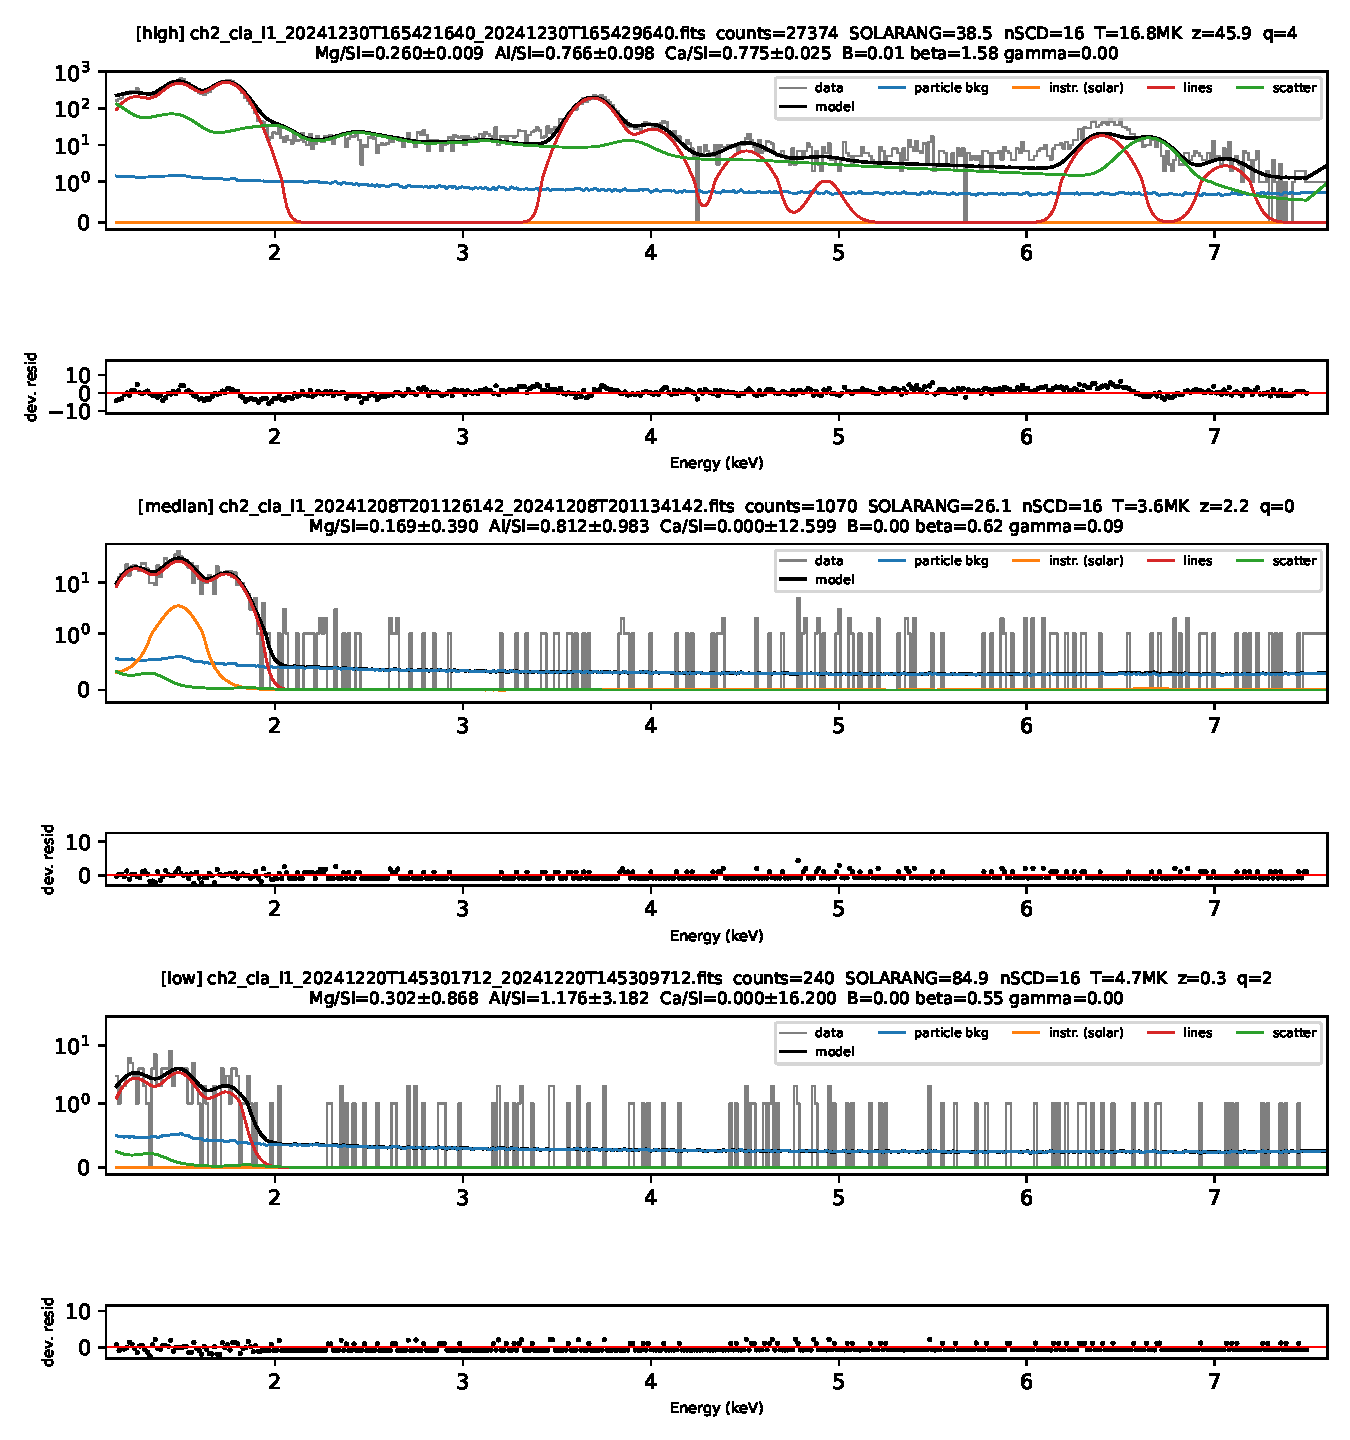
\includegraphics[width=\textwidth]{figures/fig_fits.pdf}
\caption{Example spectral fits. Fits to (a) a bright, (b) a median and (c) a faint dayside spectrum from December 2024: data (grey steps), total model (black), fluorescence lines (orange, solid), scattered solar spectrum (purple, dotted) and particle background (blue, dashed), each with deviance residuals below. The annotation in each panel gives the counts in the fitted window, the GOES temperature, the goodness-of-fit $z$ and the fitted Mg/Si and Al/Si with their $1\sigma$ uncertainties.}\label{fig:fits}
\end{figure*}

\subsection{Global maps}\label{sec:maps}
\Cref{fig:maps} shows the Mg/Si and Al/Si maps with their observation-count and standard-error layers. Over the mapping set, the median footprint ratios are Mg/Si $=\MedMg$ (5th--95th percentile \PfiveMg--\PninetyfiveMg) and Al/Si $=\MedAl$ (\PfiveAl--\PninetyfiveAl). The Mg/Si range lies within the range of returned lunar soils. The Al/Si median is higher than most returned soils, which may indicate a residual efficiency or calibration offset between the Al and Si lines (\cref{sec:limitations}). An offset of this kind would scale all values without changing the spatial pattern or the correlations, so we regard the maps as relative.

Quality-0 footprints reach every 2\textdegree{} cell (\CovUsedCells\% of cells, \CovUsedArea\% of the area), and \CovFiveArea\% of the surface is covered by cells with at least five footprints. The coverage comes from the polar orbits of the 24 archives at all local times, not from interpolation. The polar cells have the fewest footprints and the largest standard errors.

The Mg/Si map shows the expected first-order dichotomy: higher values over the nearside maria and the South Pole--Aitken basin, lower values over the farside feldspathic highlands. The Al/Si map shows the complementary pattern at higher contrast. Several maria (Imbrium, Serenitatis, Crisium, Tranquillitatis, Fecunditatis, Nubium, Humorum) and the South Pole--Aitken basin appear as low-Al/Si units against the feldspathic highlands. Residual north--south striping follows individual orbits. We attribute it mainly to orbit-to-orbit differences in the solar state that the GOES isothermal temperature does not fully capture (\cref{sec:discussion}).

\begin{figure*}[!tp]
\centering
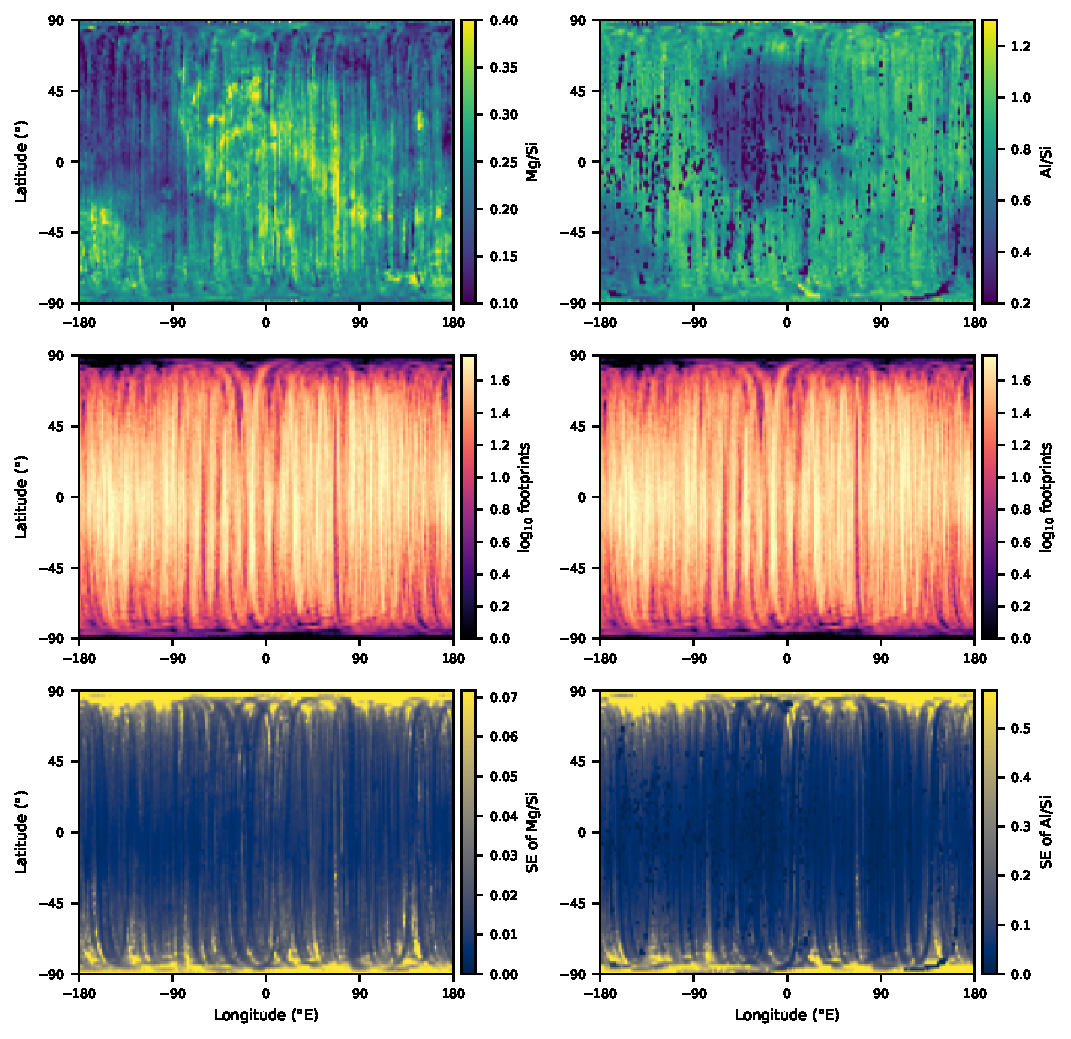
\includegraphics[width=\textwidth]{figures/fig_maps.pdf}
\caption{Global Mg/Si and Al/Si maps with quality layers. Mg/Si (left) and Al/Si (right) weight ratios on a 2\textdegree{} grid (inverse-variance-weighted means of quality-0 footprints; no smoothing or infill), with the number of footprints per cell (middle) and the standard error of the cell mean (bottom).}\label{fig:maps}
\end{figure*}

\section{Validation}\label{sec:validation}

All validation choices were fixed and logged before the first comparison:
\begin{itemize}
\item the matching radii (1, 2 and 5\textdegree, with 2\textdegree{} primary);
\item the statistics (Pearson and Spearman coefficients with bootstrap 95\% confidence intervals, leave-one-site-out ranges, and spatial block bootstrap for GRS);
\item the criterion for claiming an element as validated: Pearson $r>0$ with a 95\% confidence interval excluding zero in both the landing-site and GRS tests.
\end{itemize}
One defect was found after the first comparison and corrected; it is described at the end of this section, and both sets of numbers are reported.

\subsection{Landing sites}\label{sec:sites}
\Cref{tab:sites} lists the returned-soil ratios (average soil compositions; \citealp{Heiken1991}, Table 7.15; \citealp{Basu1998}) and the CLASS weighted means within 2\textdegree{} (\SiteFpMin--\SiteFpMax{} footprints per site).
\begin{itemize}
\item \emph{Mg/Si, 2\textdegree:} $r=\SiteMgTwoR$ (95\% CI \SiteMgTwoCI), leave-one-out range \SiteMgTwoLooLo--\SiteMgTwoLooHi, RMSE \SiteMgTwoRmse, bias \SiteMgTwoBias.
\item \emph{Al/Si, 2\textdegree:} $r=\SiteAlTwoR$ (\SiteAlTwoCI), Spearman $\rho=\SiteAlTwoRho$ ($p=\SiteAlTwoRhoP$), leave-one-out range \SiteAlTwoLooLo--\SiteAlTwoLooHi, RMSE \SiteAlTwoRmse, bias \SiteAlTwoBias.
\item \emph{1\textdegree:} Mg/Si $r=\SiteMgOneR$, Al/Si $r=\SiteAlOneR$.
\item \emph{5\textdegree:} Mg/Si $r=\SiteMgFiveR$, Al/Si $r=\SiteAlFiveR$.
\end{itemize}
The CLASS site means have small statistical errors (\cref{tab:sites}). Their scatter about the soil values is therefore systematic. Footprints of $25\times37$\,km average over terrain far larger than the sampled landing sites, several sites lie on mare--highland contacts (Apollo 15, 16, 17; Luna 20), and the instability of $r$ with radius is what one expects for nine points under these conditions. No element meets the pre-registered landing-site criterion. With $n=9$, a 95\% interval excludes zero only for $r\gtrsim0.67$.

\begin{table}[t]
\centering
\caption{Landing-site validation at 2\textdegree{} radius: returned-soil weight ratios \citep{Heiken1991} and CLASS weighted means $\pm$ standard error.}\label{tab:sites}
\begin{tabular}{lrrrrrr}
\toprule
Site & Lat & Lon & \multicolumn{2}{c}{Mg/Si} & \multicolumn{2}{c}{Al/Si}\\
 & (\textdegree) & (\textdegree E) & soil & CLASS & soil & CLASS\\
\midrule
Apollo 11 & 0.67 & 23.47 & 0.238 & 0.304$\pm$0.005 & 0.365 & 0.596$\pm$0.021\\
Apollo 12 & -3.01 & -23.42 & 0.259 & 0.285$\pm$0.006 & 0.316 & 0.473$\pm$0.014\\
Apollo 14 & -3.65 & -17.47 & 0.252 & 0.327$\pm$0.003 & 0.410 & 0.609$\pm$0.010\\
Apollo 15 & 26.13 & 3.63 & 0.317 & 0.332$\pm$0.007 & 0.353 & 0.162$\pm$0.011\\
Apollo 16 & 8.97 & 15.50 & 0.163 & 0.305$\pm$0.006 & 0.687 & 0.528$\pm$0.023\\
Apollo 17 & 20.19 & 30.77 & 0.311 & 0.321$\pm$0.007 & 0.448 & 0.655$\pm$0.018\\
Luna 16 & -0.68 & 56.30 & 0.272 & 0.308$\pm$0.005 & 0.415 & 0.609$\pm$0.015\\
Luna 20 & 3.53 & 56.55 & 0.280 & 0.297$\pm$0.004 & 0.560 & 0.745$\pm$0.017\\
Luna 24 & 12.71 & 62.20 & 0.276 & 0.307$\pm$0.004 & 0.322 & 0.397$\pm$0.012\\
\bottomrule
\end{tabular}

\end{table}

\subsection{Lunar Prospector GRS}\label{sec:grs}
On the 5\textdegree{} equal-area GRS pixels, all \GrsMgN{} of which contain at least 20 CLASS footprints:
\begin{itemize}
\item \emph{Mg/Si:} $r=\GrsMgR$ (block-bootstrap 95\% CI \GrsMgCI; Spearman $\rho=\GrsMgRho$);
\item \emph{Al/Si:} $r=\GrsAlR$ (\GrsAlCI; $\rho=\GrsAlRho$).
\end{itemize}
Both pass the GRS criterion (\cref{fig:validation}). The correlations are stable under the count-threshold sensitivity test: Mg/Si $r=\GrsMgR$, \GrsMgRMinK, \GrsMgRMinKKK{} and Al/Si $r=\GrsAlR$, \GrsAlRMinK, \GrsAlRMinKKK{} for thresholds of 300, 1000 and 3000 counts (\NMapped, \NMappedMinK{} and \NMappedMinKKK{} spectra). The GRS Mg and Al abundances themselves carry substantial model-dependent uncertainty \citep{Prettyman2006}, so these correlations are lower bounds on the agreement achievable.

\begin{figure}[t]
\centering
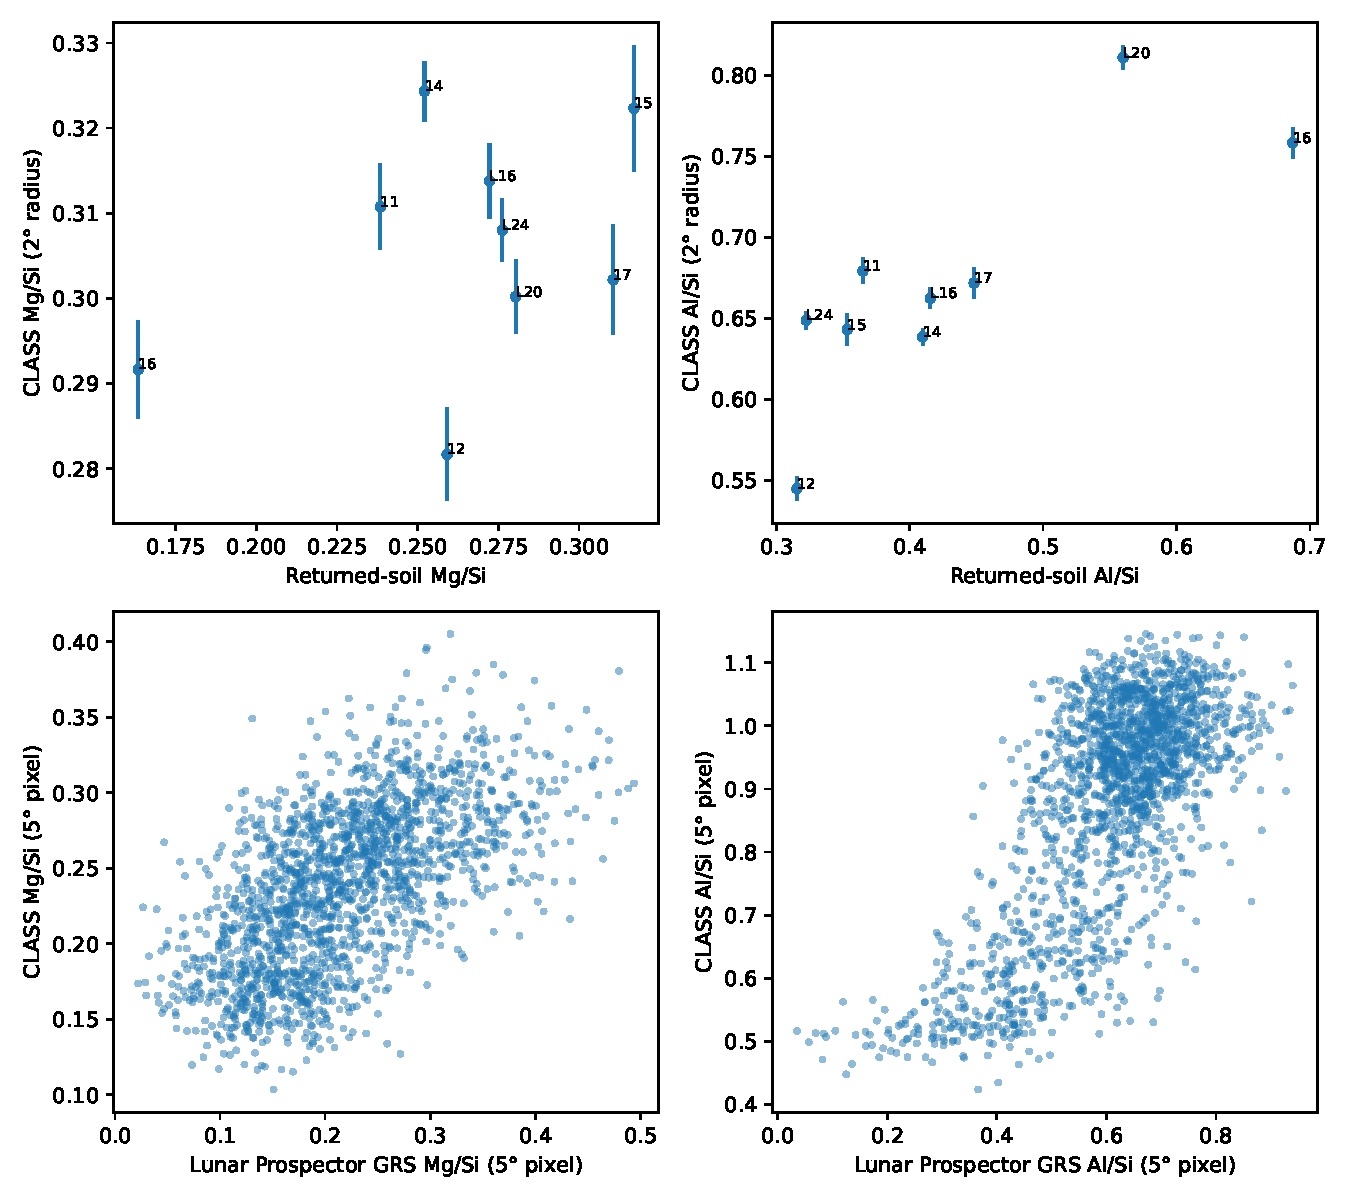
\includegraphics[width=\textwidth]{figures/fig_validation.pdf}
\caption{Top: CLASS ratios within 2\textdegree{} of the landing sites against returned-soil ratios. Bottom: CLASS against Lunar Prospector GRS ratios on 5\textdegree{} equal-area pixels.}\label{fig:validation}
\end{figure}

\subsection{Disclosed post-validation correction}\label{sec:fix}
The first comparison produced a population of Al/Si values near zero. These were 254 fits (0.06\% of the mapping set) in which the instrumental component had absorbed the Al line. Their Al/Si estimates of $\sim10^{-5}$ lay just above the boundary threshold of $10^{-6}$ used to flag pinned parameters. A Fisher-matrix uncertainty is meaningless at a boundary, and theirs had collapsed below $10^{-3}$, so these fits carried 93\% of the total inverse-variance weight. Raising the boundary threshold to $10^{-3}$, below any lunar Mg/Si or Al/Si, removes them.

The pre-correction results were GRS Al/Si $r=\GrsAlRvOne$ (\GrsAlCIvOne), Mg/Si unchanged, and landing-site correlations within 0.02 of the values above. We regard this as a bug fix, not a tuning step, but report it so that readers can judge.

\subsection{What limits the scores?}\label{sec:limits_scores}
Several diagnostics, computed after the pre-registered tests and changing none of them, explain the size of the correlations.

\emph{The landing-site test has little discriminating power at this scale.} Applied to the same nine soil averages, using the 5\textdegree{} pixel containing each site, the Lunar Prospector GRS itself gives $r=\GrsSitesMg$ for Mg/Si and $\GrsSitesAl$ for Al/Si. Site-average soils sample metres to kilometres around each landing point, while orbital pixels average tens to hundreds of kilometres of terrain on mare--highland contacts \citep{Basu1998}. A small or negative $r$ in this test therefore says little about map quality.

\emph{The GRS correlation is bounded by the noise in both data sets.} We split the mapping set into two halves by alternate months, map each half separately, and correlate the two maps. After Spearman--Brown correction, this gives a reliability of the CLASS pixel means of \RelMg{} for Mg/Si and \RelAl{} for Al/Si. The GRS error matrices imply reliabilities of \RelGrsMg{} and \RelGrsAl. The maximum attainable correlation is therefore $\sqrt{\rho_\mathrm{CLASS}\rho_\mathrm{GRS}}=\CeilMg$ for Mg/Si and \CeilAl{} for Al/Si. The observed $r=\GrsMgR$ for Mg/Si is close to its ceiling. For comparison, the earlier processing of the same data gives $r=\OldGrsMg$ and \OldGrsAl{} on the same pixels.

\emph{Al/Si is limited by the instrumental component.} The low split-half reliability of Al/Si comes from month-to-month offsets. In a fixed farside equatorial region, the monthly median Al/Si anticorrelates with the fraction of spectra in which the fitted instrumental amplitude $\gamma$ is non-zero (Spearman $-0.88$). In a few months the free $\gamma$ absorbs part of the lunar Al line.

\paragraph{Post-hoc analyses (labelled as such)} Two variants were examined after validation; neither replaces the pre-registered product.
\begin{itemize}
\item \emph{Weighted median.} Replacing the weighted mean by a weighted median does not help: GRS $r=\MedGrsMg$ (Mg/Si) and \MedGrsAl{} (Al/Si), Al/Si reliability \MedRelAl.
\item \emph{Spectra with $\gamma\approx0$.} The nightside data imply that the instrumental component should be negligible on the dayside (\cref{fig:background}). Restricting the maps to spectra with fitted $\gamma<0.05$ (\GzN{} spectra, \GzPct\% of the mapping set) raises the Al/Si reliability to \GzAlRel. Against GRS, Al/Si then gives $r=\GzAlR$ (\GzAlCI) and Mg/Si $r=\GzMgR$ (\GzMgCI). Against the landing sites at 2\textdegree, Al/Si gives $r=\GzSiteAlR$ (\GzSiteAlCI) and Mg/Si $r=\GzSiteMgR$; the Al/Si site results at 1\textdegree{} and 5\textdegree{} are \GzSiteAlROne{} and \GzSiteAlRFive.
\end{itemize}
The $\gamma$ cut uses a fitted model parameter, not the reference data. It does, however, select spectra after the fact, and its median Al/Si (\GzAlMed) is higher than that of the full set. We therefore present it as evidence that the instrumental-aluminium degeneracy, rather than the fluorescence model, limits Al/Si. A model in which $\gamma$ is fixed to zero on the dayside, specified in advance, is the natural next step. \Cref{fig:posthoc} shows the weighted-median alternative maps.

\begin{figure}[t]
\centering
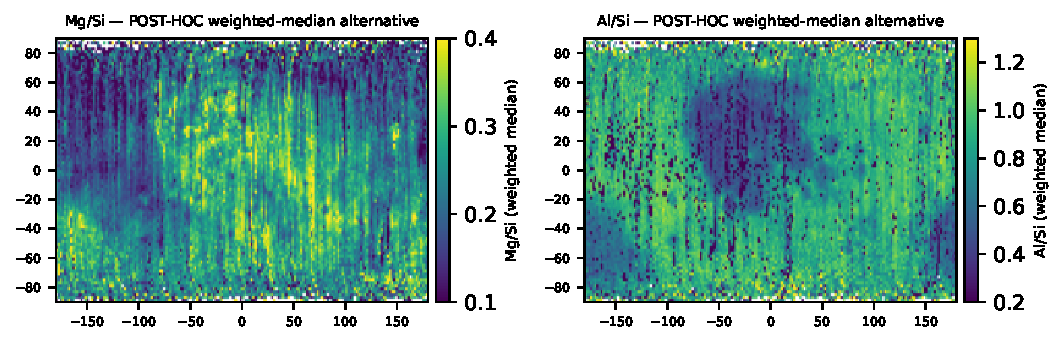
\includegraphics[width=\textwidth]{figures/fig_maps_wmedian_posthoc.pdf}
\caption{\textbf{Post-hoc alternative (not the pre-registered product):} inverse-variance-weighted median of footprint ratios per 2\textdegree{} cell (footprint centres).}\label{fig:posthoc}
\end{figure}

\subsection{Outcome}
Under the pre-registered rule, neither element is claimed as validated: both pass the GRS test, and both fail the nine-site test, which has little statistical power at this footprint size. We therefore present Mg/Si and Al/Si as relative maps whose large-scale pattern agrees with an independent orbital data set, strongly for Mg/Si and moderately for Al/Si, and we make no claim of site-level accuracy. The post-hoc analysis of \cref{sec:limits_scores} indicates that Al/Si can reach a GRS correlation of \GzAlR{} once the instrumental-aluminium degeneracy is controlled.

\section{Discussion}\label{sec:discussion}

\subsection{Why the solar spectrum matters for line ratios}
Ratios to Si are often treated as insensitive to the incident spectrum. Our forward model shows that they are not. Each K line is excited by the part of the solar spectrum above its own edge (Mg \SI{1.31}{keV}, Si \SI{1.84}{keV}, Ca \SI{4.04}{keV}), and at coronal temperatures that part is dominated by a few He-like line complexes whose relative strengths change steeply with temperature.

In our synthetic tests, a 30\% hotter spectrum than assumed biases Mg/Si by \SynHotMg\% and changes Ca/Si by an order of magnitude. Refitting real data with the GOES temperature scaled by 0.8 and 1.2 changes the median Mg/Si by \TsensMgLo\% and \TsensMgHi\%, and Al/Si by \TsensAlLo\% and \TsensAlHi\%.

Before the solar lines were included, a continuum-only reference spectrum with any single temperature produced Mg/Si values of 0.3--0.8 together with Ca/Si of 0.004--0.5, never simultaneously lunar. The implausible ratios of earlier CLASS processing (Mg/Si $\approx1.4$, Ca/Si $\approx0.01$) have the same origin. A time-resolved description of the solar spectrum is therefore not an optional refinement but a requirement, even for ratio maps.

\subsection{GOES as a proxy for the solar spectrum}
GOES provides the solar state for every CLASS exposure from public data. Its limitations are well known. The two-channel temperature is a single isothermal value. It is weighted towards the hottest plasma. Below the B1 level it is unreliable, and we found it pinned to the edge of the response table or diverging there. The GOES-16 and GOES-18 temperatures agree to 0.5\% in their overlap.

The real corona is multi-thermal. The isothermal approximation underpredicts the flux above \SI{4}{keV} at the temperatures typical of our data. This is why Ca/Si is biased even in self-consistent synthetic tests, and why Ti and Fe cannot be constrained at all. The residual orbit-to-orbit striping in the maps is consistent with solar-state errors of this kind. XSM spectra measured simultaneously with CLASS \citep{Mithun2020} would remove this limitation, and our model accepts any tabulated $S(E)$, so the extension is direct.

\subsection{The instrumental aluminium component}
The Al K$\alpha$ excess in sunlit nightside spectra has a sharp onset near \texttt{SOLARANG} $\approx93^\circ$ and disappears at the shadow boundary (\cref{fig:background}). It must therefore be excited by solar X-rays that reach aluminium in the instrument (filters, frames, housing; \citealp{Pillai2021}) when the Sun is behind the spacecraft. On the dayside the Sun is in front of the nadir-pointing instrument, and the component is absent.

Mishandling it is costly. Subtracting a month-averaged nightside spectrum, as earlier processing did, removes a time-variable amount of Al. Fitting its amplitude freely, as in our alternative model, lets it absorb lunar Al in some months; Al/Si reliability then drops from \RelAl{} to \RelAlvTwo{} and the GRS correlation from \GrsAlR{} to \GrsAlRvTwo. Other XRF instruments with aluminium structures or filters may show the same effect, and it can be identified with the same nightside test.

\subsection{Limitations}\label{sec:limitations}
\begin{enumerate}
\item \emph{No measured solar spectrum.} The solar spectrum is isothermal at the GOES temperature. In synthetic tests, temperature errors of $+30$\% and $-20$\% bias Mg/Si by \SynHotMg\% and \SynColdMg\%, and Al/Si by \SynHotAl\% and \SynColdAl\%. Scaling the GOES temperature of real data by 0.8 and 1.2 changes Mg/Si by \TsensMgLo\% and \TsensMgHi\% (\cref{sec:synthetic}). Ca/Si, Ti/Si and Fe/Si are not retrievable.
\item \emph{Relative, not absolute.} The products are weight ratios to Si. No absolute calibration is attempted, and the amplitude $A$ absorbs the solar flux, area and geometry.
\item \emph{Detector efficiency.} The published filter transmission is applied. The SCD quantum efficiency and any surface dead layer are not modelled, because no curve is published. This mainly affects the Si line relative to Mg and Al, and probably explains why the median Al/Si (\MedAl) is higher than most returned soils. Such an offset rescales the maps but leaves their pattern and correlations unchanged.
\item \emph{Physical effects not modelled.} Particle-size and roughness effects, phase-angle dependence beyond the plane-parallel geometry, and the angular dependence of scattering are not modelled.
\item \emph{Spatial resolution.} Footprints are $25\times37$\,km. The maps are 2\textdegree{} and should not be interpreted at finer scales.
\item \emph{Small validation sample.} Nine landing sites, sampled at the scale of a footprint, give a test with little statistical power. The GRS comparison is limited by the GRS resolution and by its own model dependence for Mg and Al.
\end{enumerate}

\section{Conclusions}\label{sec:conclusions}

We have described a CLASS processing chain that uses only public data. It combines a simplified fundamental-parameter model, a CHIANTI solar spectrum at the GOES temperature of each exposure, the published filter transmission, a particle-background template and a Poisson likelihood fit with per-spectrum uncertainties and quality flags. Applied to \NRawFiles{} Level-1 exposures from \NMonths{} monthly archives, it gives \NMapped{} quality-controlled spectra and global 2\textdegree{} maps of Mg/Si and Al/Si with complete observed coverage. Our main findings are:
\begin{enumerate}
\item Element/Si ratios depend appreciably on the incident solar spectrum. Solar line emission carries most of the flux that excites Mg, Al and Si, and an isothermal spectrum at the GOES temperature brings the retrieved Mg/Si into the lunar range.
\item CLASS nightside spectra contain a solar-driven instrumental Al K$\alpha$ component when the Sun illuminates the spacecraft from behind. How it is treated in the dayside background model affects Al/Si.
\item With a GOES-based solar spectrum, Mg/Si and Al/Si can be recovered, whereas Ca/Si, Ti/Si and Fe/Si are dominated by solar-spectrum systematics.
\item Al/Si agrees with Lunar Prospector GRS ($r=\GrsAlR$) and with nine landing-site soils ($r=\SiteAlTwoR$), and several maria appear as distinct units. Mg/Si agrees with GRS ($r=\GrsMgR$); its landing-site comparison is inconclusive, as it is for GRS itself.
\item For three months, replacing the GOES-based spectrum by XSM-derived spectra changes the median Al/Si by a few per cent and Mg/Si by \XsmTwoMg{} to \XsmOneMg\%, depending on the assumed thermal structure. This supports Al/Si as the more robust product and identifies the solar spectrum as the main uncertainty for Mg/Si.
\end{enumerate}
The code, mapping-set results and maps are public. Extending the XSM-based treatment to all months, with free coronal abundances, is the most direct way to reduce the remaining systematic uncertainty.


\appendix
\setcounter{table}{0}
\setcounter{figure}{0}
\section{Per-month statistics and calibration}\label{app:months}
Table~\ref{tab:months} lists the per-month exposure counts, mapping-set size, fitted energy-scale parameters and the source of the particle template.

\begin{table}[!h]
\centering
\tiny
\setlength{\tabcolsep}{2pt}
\caption{Per-month exposure counts, mapping-set size, fitted energy-scale parameters and particle-template source.}\label{tab:months}
\begin{tabular}{lrrrrrrl}
\toprule
Month & Files & Dayside & Mapped & $g$ (eV/ch) & $o$ (eV) & FWHM$_{1.49}$ (eV) & Umbra template\\
\midrule
2020-12 & 3{,}931 & 3{,}051 & 94 & 13.379 & 29.3 & 107 & own\\
2021-01 & 4{,}634 & 3{,}501 & 0 & 13.383 & 13.7 & 108 & own\\
2021-02 & 40{,}247 & 27{,}555 & 546 & 13.896 & -24.4 & 92 & own\\
2022-03 & 5{,}896 & 2{,}793 & 731 & 13.717 & 1.1 & 119 & Dec 2024\\
2024-03 & 15{,}076 & 7{,}939 & 1{,}982 & 13.678 & 8.6 & 119 & Dec 2024\\
2024-11 & 104{,}125 & 74{,}962 & 51{,}815 & 13.759 & 1.1 & 165 & own\\
2024-12 & 97{,}345 & 75{,}720 & 42{,}704 & 13.737 & 2.2 & 185 & own\\
2025-01 & 51{,}298 & 38{,}780 & 27{,}580 & 13.740 & 3.1 & 162 & own\\
2025-02 & 92{,}570 & 63{,}780 & 44{,}826 & 13.739 & 3.6 & 156 & own\\
2025-03 & 40{,}571 & 20{,}519 & 4{,}606 & 13.765 & 0.7 & 145 & own\\
2025-04 & 81{,}585 & 48{,}469 & 18{,}672 & 13.839 & -6.5 & 145 & own\\
2025-05 & 94{,}521 & 65{,}910 & 39{,}426 & 13.634 & 16.1 & 156 & own\\
2025-06 & 97{,}669 & 68{,}095 & 48{,}494 & 13.819 & -5.8 & 168 & own\\
2025-07 & 90{,}614 & 67{,}190 & 44{,}079 & 13.641 & 15.7 & 161 & own\\
2025-08 & 97{,}593 & 66{,}706 & 39{,}325 & 13.821 & -5.9 & 156 & own\\
2025-09 & 40{,}747 & 23{,}210 & 11{,}039 & 13.898 & -13.2 & 151 & own\\
2025-10 & 27{,}237 & 16{,}137 & 2{,}018 & 13.684 & 9.4 & 169 & own\\
2025-11 & 105{,}203 & 74{,}667 & 41{,}296 & 13.700 & 8.0 & 169 & own\\
2025-12 & 92{,}318 & 71{,}126 & 44{,}952 & 13.747 & 3.3 & 176 & own\\
2026-01 & 85{,}725 & 65{,}896 & 43{,}891 & 13.856 & -8.1 & 176 & own\\
2026-02 & 84{,}922 & 61{,}436 & 24{,}301 & 13.738 & 7.0 & 156 & own\\
2026-03 & 31{,}184 & 18{,}295 & 2{,}913 & 13.669 & 15.1 & 160 & own\\
2026-04 & 29{,}064 & 16{,}453 & 5{,}528 & 13.821 & 0.8 & 148 & own\\
2026-05 & 101{,}164 & 71{,}799 & 37{,}712 & 13.766 & 7.9 & 155 & own\\
\bottomrule
\end{tabular}

\end{table}

\section*{Data availability}
CLASS Level-1 data \citep{CLASSdata} and XSM data \citep{XSMdata} are available from the ISRO PRADAN portal. GOES XRS 1-minute science-quality data are available from NOAA/NCEI \citep{GOESdata}. The Lunar Prospector GRS elemental abundances are available from the PDS Geosciences Node \citep{PrettymanPDS2012}. The processing code, the per-footprint results of the mapping set, the maps and the scripts that generate every number and figure in this paper are available at \url{https://github.com/GeeteshPaidi/SomaDhatuNirupana} and archived on Zenodo \citep{SomaDhatu}.


\section*{Declaration of competing interest}
The authors declare that they have no known competing financial interests or personal relationships that could have appeared to influence the work reported in this paper.

\section*{Funding}
This research did not receive any specific grant from funding agencies in the public, commercial, or not-for-profit sectors.

\section*{Declaration of generative AI and AI-assisted technologies in the manuscript preparation process}
During the preparation of this work the authors used Claude (Anthropic) in order to assist with code development, data analysis, and drafting and editing of the manuscript text. After using this tool, the authors reviewed and edited the content as needed and take full responsibility for the content of the published article.

\section*{Acknowledgements}
We thank ISRO/ISSDC for public access to Chandrayaan-2 CLASS and XSM data through PRADAN, the XSM Payload Operations Centre (Physical Research Laboratory) for the XSM data products and calibration database, NOAA/NCEI for GOES XRS science-quality data, and the PDS Geosciences Node for the Lunar Prospector GRS products. This research used the open-source packages xraylib, SunPy, sunkit-instruments, sunkit-spex, NumPy, SciPy and Astropy.

\bibliographystyle{elsarticle-harv}
\bibliography{references}

\end{document}
